\section{Securely destroying data}

Just hit the delete button and you are done! No it's not that easy. To
understand how to securely delete data, we have to understand how data
is stored. In an analogy to the real world, an explanation of how data
is stored follows:

Assume you have a small notebook with 10 pages and you want to write
some data in this notebook. You just start writing on the first page up
to the end of the notebook. Maybe you decide the information on page 5
must be destroyed. Probably you will just take out the page and burn it.

Unfortunately data on a harddisk doesn't work this way. A harddisk
contains not ten but thousands or maybe even millions of pages. Also
it's impossible to take out a ``page'' of a harddisk and destroy it. To
explain how a harddisk work, we will continue with our 10-page notebook
example. But now we will work a little bit different with it. We will
work in a way similar to how a harddisk works.

This time we use the first page of our notebook as an index. Assume we
write a piece about ``WikiLeaks'', then on the first page we write a
line ``piece about WikiLeaks: see page 2''. The actual piece is then
written on page 2.

For the next document, a piece about ``Goldman Sachs'' we add a line on
page 1, ``Goldman Sachs: see page 3''. We can continue this way till our
notebook is full. Let's assume the first page will look like this:

\begin{itemize}
\item
  WikiLeaks -\textgreater{} see page 2
\item
  Goldman Sachs -\textgreater{} see page 3
\item
  Monstanto scandal -\textgreater{} see page 4
\item
  Holiday pictures -\textgreater{} see page 5
\item
  KGB Investigation -\textgreater{} see page 6
\item
  Al Jazeeraa contacts -\textgreater{} see page 7
\item
  Iran nuclear program -\textgreater{} see page 8
\item
  Sudan investigation -\textgreater{} see page 9
\item
  Infiltration in EU-politics -\textgreater{} see page 10
\end{itemize}
Now, let's decide you want to wipe the ``Goldman Sachs'' piece, what a
harddisk will do, it will only remove the entry on the first page, but
not the actual data, your index will be:

\begin{itemize}
\item
  WikiLeaks -\textgreater{} see page 2
\item
  Monstanto scandal -\textgreater{} see page 4
\item
  Holiday pictures -\textgreater{} see page 5
\item
  KGB Investigation -\textgreater{} see page 6
\item
  Al Jazeeraa contacts -\textgreater{} see page 7
\item
  Iran nuclear program -\textgreater{} see page 8
\item
  Sudan investigation -\textgreater{} see page 9
\item
  Infiltration in EU-politics -\textgreater{} see page 10
\end{itemize}
What we did, we removed only the reference to the article, but if we
open page 3, we will still able to read the Goldman Sachs piece. This is
exactly the way what a harddisk does when your ``delete'' a file. With
specialized software it still able to ``recover'' page 3.

To securely delete data, we should do the following:

\begin{enumerate}[1.]
\item
  Open the ``Goldman Sachs'' page (page 3)
\item
  Use an eraser to remove the article there, if done return to page 1
\item
  Delete the reference in the index on page 1
\end{enumerate}
Well you will be surprised by the similarity between this example and
the real world. You know when you removed the article on page 3 with an
eraser, it is still possible to read the article slightly. The pencil
leaves a track on the paper because of the pressure of the pencil on the
paper and also you will be unable to erase all of the graphite. Small
traces are left behind on the paper. If you really need this article,
you can reconstruct (parts) of it, even if it's erased.

With a harddisk this is very similar. Even if you erased every piece of
data, it is sometimes possible with (very) specialized hardware to
recover pieces of the data. If the data is very confidential and must be
erased with the greatest care, you can use software to ``overwrite'' all
pieces of data with random data. When this is done multiple times, this
will make the data untraceable.

\subsection{A note on Solid State Hard Drives}

The instructions below explain how to use file deletion tools to
securely delete files from your hard drives. These tools rely on the
Operating System you are using being able to directly address every byte
on the hard drive in order to tell the drive ``set byte number X to 0''.
Unfortunately, due to a number of advanced technologies used by Solid
State Drives (SSDs) such as TRIM, it is not always possible to ensure
with 100\% certainty that every part of a file on an SSD has been erased
using the tools below.

\subsection{Securely delete data under Windows}

For Windows there is a good open source tool called ``File Shredder''.
This tool can be downloaded from http://www.fileshredder.org

The installation is very straightforward, just download the application
and install it by hitting the next button. After installation this
application will automatically start. You can then start using it for
shredding files. However the best part of the program is that you can
use it from within windows itself by right clicking on a file.

\begin{enumerate}[1.]
\item
  Click right on the file you want to shred, and choose File Shredder
  -\textgreater{} Secure delete files
\end{enumerate}
\begin{figure}[htbp]
\centering
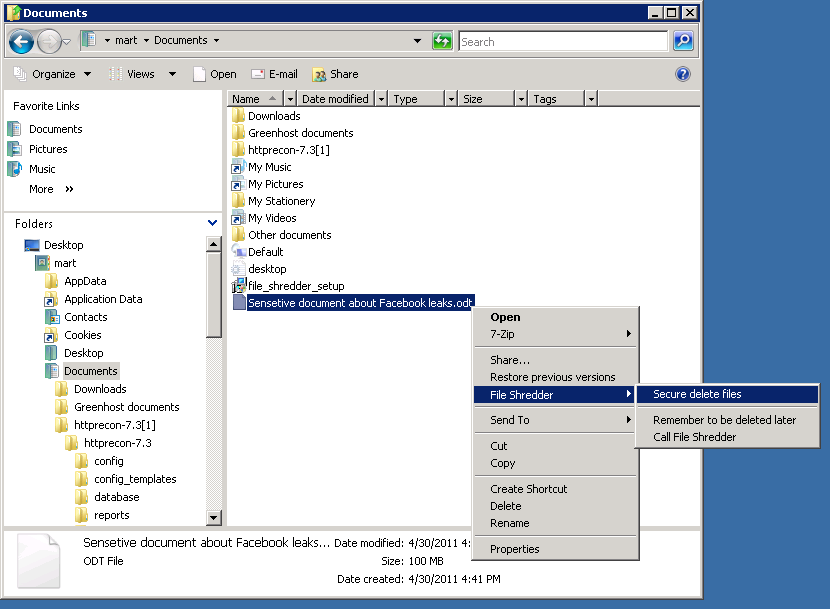
\includegraphics{destroy_data_001.png}
\caption{Destroying data}
\end{figure}

\begin{enumerate}[1.]
\setcounter{enumi}{1}
\item
  A pop-up asks if you really want to shred this file
\end{enumerate}
\begin{figure}[htbp]
\centering
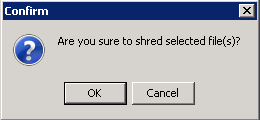
\includegraphics{destroy_data_002.png}
\caption{Destroying data}
\end{figure}

\begin{enumerate}[1.]
\setcounter{enumi}{2}
\item
  After confirming, there your file goes. Depending on the size of the
  file this can take a while
\end{enumerate}
\begin{figure}[htbp]
\centering
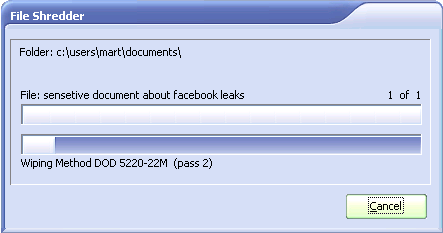
\includegraphics{destroy_data_003.png}
\caption{Destroying data}
\end{figure}

\subsection{Securely delete data under MacOSX}

There are basically to build-in steps to make to securely delete your
data on Mac OSX.

\begin{enumerate}[1.]
\item
  Erase the free-space on your hard-drive containing all the data of
  items which are deleted in an insecure way.
\item
  Make sure that every file from then on is always securely deleted.
\end{enumerate}
We start with the first one:

\subsubsection{Erasing Free Space}

\begin{enumerate}[1.]
\item
  Open Disk-Utility which resides in the Utilities folder inside the
  Applications folder.
\end{enumerate}
\begin{figure}[htbp]
\centering
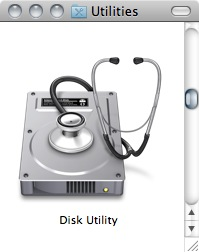
\includegraphics{destroy_data_004.jpg}
\caption{Destroying data}
\end{figure}

\begin{enumerate}[1.]
\setcounter{enumi}{1}
\item
  Select your hard drive and click on `Erase Free Space'.
\end{enumerate}
\begin{figure}[htbp]
\centering
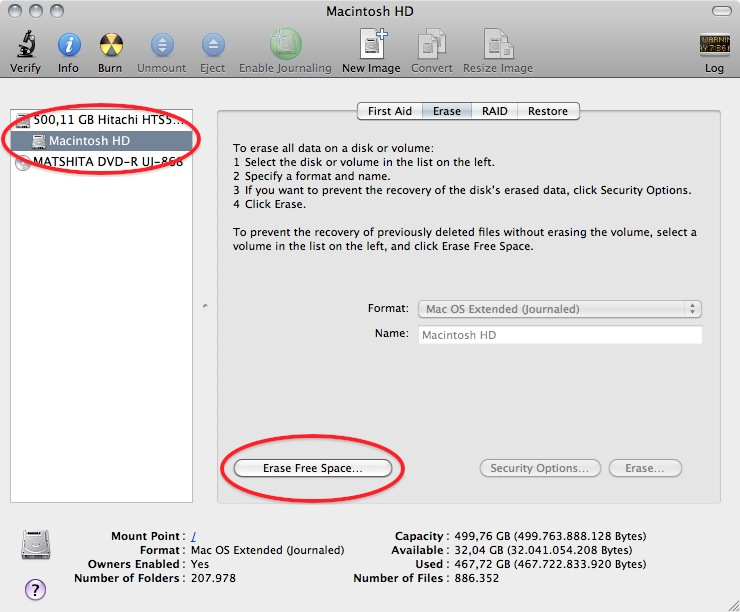
\includegraphics{destroy_data_005.jpg}
\caption{Destroying data}
\end{figure}

\begin{enumerate}[1.]
\setcounter{enumi}{2}
\item
  Three options will appear, from top to bottom more secure, but also
  they take much more time to complete. Read the descriptions on each
  one of them to get an idea from what will happen if you use them and
  then choose which one might suite your needs the best and click `Erase
  free Space'.
\end{enumerate}
If time is no issue, then use the most secure method and enjoy your free
time to get a good coffee while you Mac crunches away on this task. If
the crooks are already knocking on your front-door you might want to use
the fastest way.

\begin{figure}[htbp]
\centering
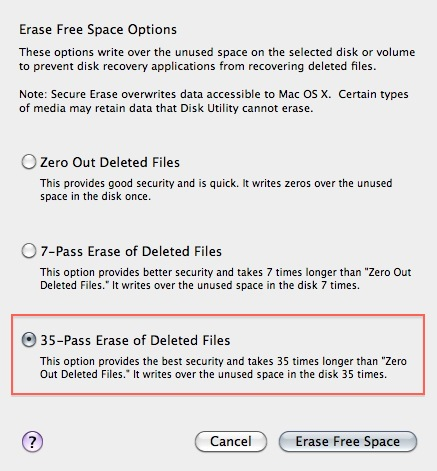
\includegraphics{destroy_data_006.jpg}
\caption{Destroying data}
\end{figure}

\subsubsection{Securely Erasing Files}

Now that your previously deleted data is once and for ever securely
erased you should make sure that you don't create any new data that
might be recovered at a later date.

\begin{enumerate}[1.]
\item
  To do this open the finder preferences under the Finder Menu.
\end{enumerate}
\begin{figure}[htbp]
\centering
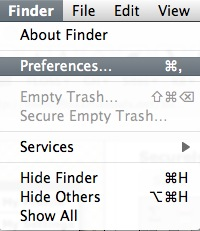
\includegraphics{destroy_data_007.jpg}
\caption{Destroying data}
\end{figure}

\begin{enumerate}[1.]
\setcounter{enumi}{1}
\item
  Go to the advanced tab and tick `Empty trash securely'. This will make
  sure that every time you empty your trash all the items in it will be
  securely deleted and are really gone!
\end{enumerate}
\begin{figure}[htbp]
\centering
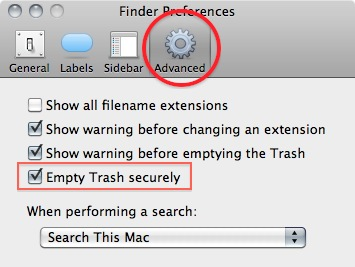
\includegraphics{destroy_data_008.jpg}
\caption{Destroying data}
\end{figure}

\textbf{Note:} Deleting your files securely will take longer then just
deleting them. If you have to erase big portions of unimportant data
(say your movie and mp3 collection) you may wanna untick this option
before doing so.

\subsection{Securely delete data under Ubuntu/Linux}

Unfortunately currently there is no graphical user interface available
for Ubuntu to delete files secure. There are two command-line programs
available though:

\begin{itemize}
\item
  shred
\item
  wipe
\end{itemize}
Shred is installed in Ubuntu by default and can delete single files.
Wipe is not installed by default but can easily be installed with using
Ubuntu Software Center or if you understand the command line you can
install it with \verb!apt-get install wipe!. Wipe is a little more
secure and has nicer options.

It is possible make access to these program's easy by adding it as an
extra menu option

\begin{enumerate}[1.]
\item
  We assume you are familiar with the Ubuntu Software Center. To add the
  securely wipe option, it's required to install these two programs
  \emph{wipe} and \emph{nautilus-actions}
\end{enumerate}
If the two programs are installed follow the following steps. If they
are not installed use the Ubuntu Software Center to install them or on
the command line simply type apt-get install nautilus-actions wipe

\begin{enumerate}[1.]
\setcounter{enumi}{1}
\item
  Open the ``Nautilus Actions Configuration'' from the System
  -\textgreater{} Preferences menu
\end{enumerate}
\begin{figure}[htbp]
\centering
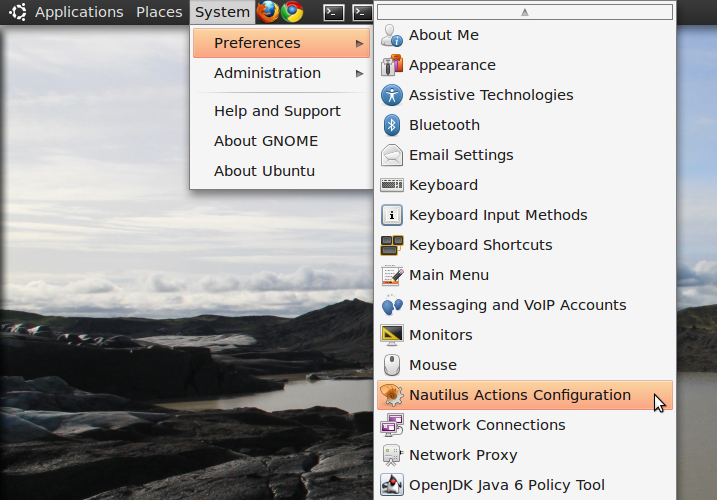
\includegraphics{destroy_data_009.png}
\caption{Destroying data}
\end{figure}

\begin{enumerate}[1.]
\setcounter{enumi}{2}
\item
  We have to add a new action. To do this, start clicking on the
  ``create new action button'', the first option in the toolbar
\end{enumerate}
\begin{figure}[htbp]
\centering
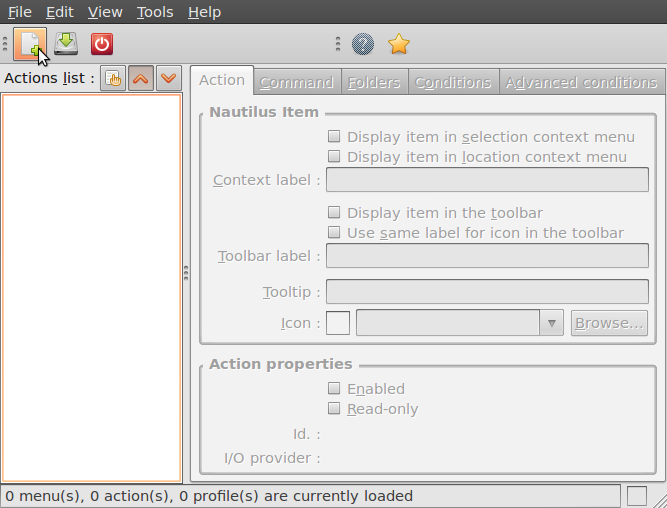
\includegraphics{destroy_data_010.png}
\caption{Destroying data}
\end{figure}

\begin{enumerate}[1.]
\setcounter{enumi}{3}
\item
  Next is describing the new action. You can give the action every name
  you wish. Fill out this title in the ``Context label'' field. In this
  example we used ``Delete file securely''
\end{enumerate}
\begin{figure}[htbp]
\centering
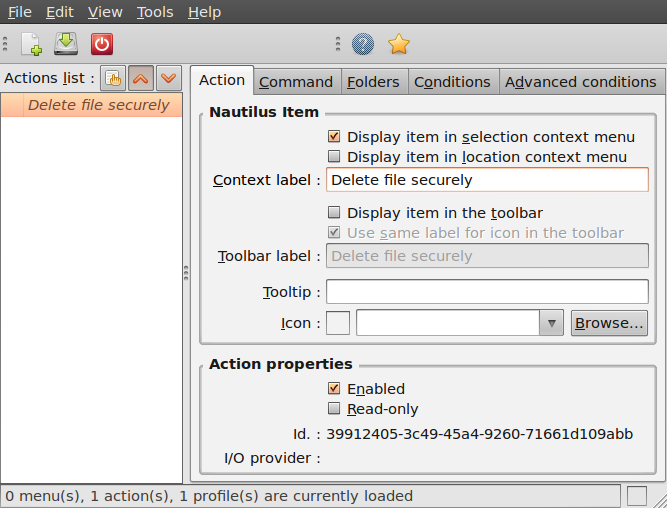
\includegraphics{destroy_data_011.png}
\caption{Destroying data}
\end{figure}

\begin{enumerate}[1.]
\setcounter{enumi}{4}
\item
  Click on the second tab (``Command''), here is how we specify the
  action we want. In the field ``Path'', type ``wipe'', in the field
  parameters type ``-rf \%M'', please be sure about the capitalisation
  of all characters here, this is very important.
\end{enumerate}
\begin{figure}[htbp]
\centering
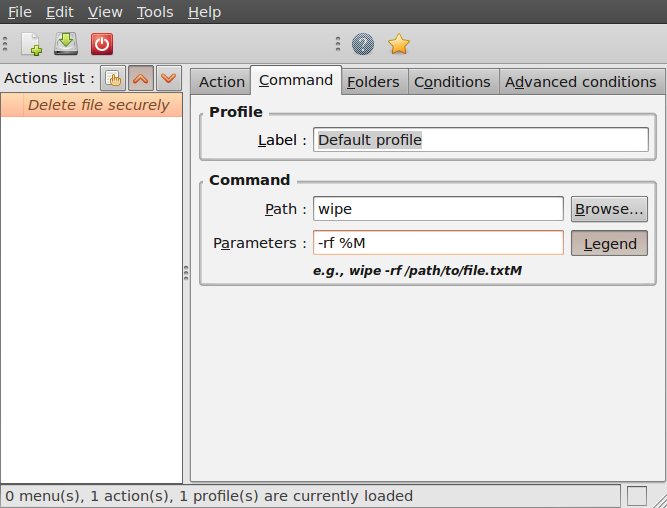
\includegraphics{destroy_data_012.png}
\caption{Destroying data}
\end{figure}

\begin{enumerate}[1.]
\setcounter{enumi}{5}
\item
  Next is specifying the conditions, click on the conditions tab and
  choose the option ``Both'' in the ``Appears if selection
  contains\ldots{}'' box. With this option you can wipe both files and
  folders securely. If done, click the save button (second item on the
  icon bottom toolbar) or use the menu File-\textgreater{}Save
\end{enumerate}
\begin{figure}[htbp]
\centering
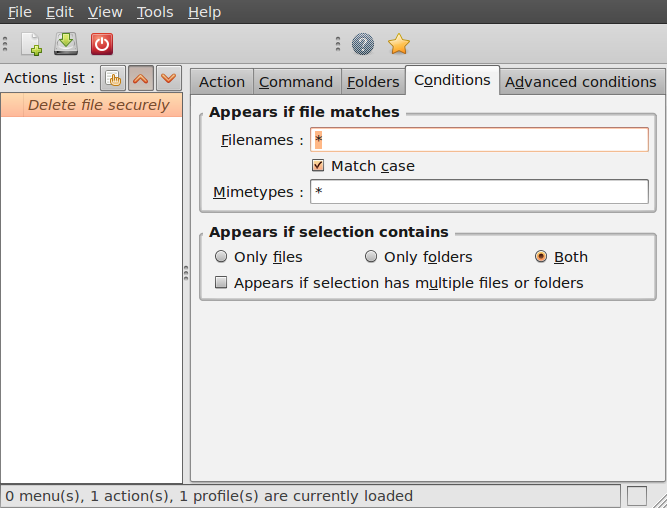
\includegraphics{destroy_data_013.png}
\caption{Destroying data}
\end{figure}

\begin{enumerate}[1.]
\setcounter{enumi}{6}
\item
  Now close the Nautilus Actions Configuration tool. Unfortunately,
  after this, you have to re-login into your system, so ether reboot or
  logout/login.
\item
  Now browse to the file you want to securely delete and right click:
\end{enumerate}
\begin{figure}[htbp]
\centering
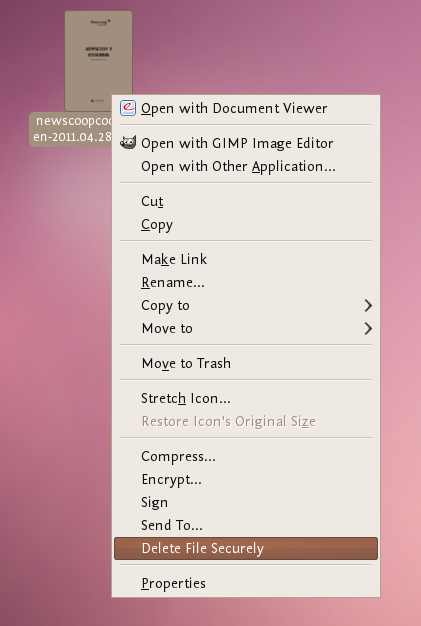
\includegraphics{destroy_data_014.png}
\caption{Destroying data}
\end{figure}

Choose `Delete File Securely'. The file will then be wiped `quietly' -
you do not get any feedback or notice that the process has started or
stopped. However the process is underway. It takes some time to securely
delete data and the bigger the file the longer it takes. When it is
complete the icon for the file to be wiped will disappear. If you would
like to add some feedback you can change the parameters field in
Nautilius Actions Configuration tool to this:

\verb!-rf %M | zenity --info --text "your wipe is underway please be patient. The icon of the file to be wiped will disappear shortly."!

The above line will tell you the process is underway but you will not
know the file is deleted until the icon disappears.
